\begin{center}
\large Experimento: \textbf{Amplificador diferencial com TJB}
\end{center}


\section{Introdução}



O presente relatório visa detalhar o experimento laboratorial realizado na disciplina laboratório de circuitos eletrônicos no dia 3 de setembro de 2019 sobre amplificador diferencial com transistores de junção bipolar (TJBs). 
 
Esse tipo de amplificador diferencial é utilizado para amplificação com rejeição de ruído devido à sua configuração diferencial, assim promovendo um sinal diferencial nas saídas dos transistores que além do benefício mencionado anteriormente, permite uma maior excursão do sinal de saída.

A prática objetiva a medição do ganho de modo comum ($A_{CM}$) e o ganho diferencial ($A_d$) de um amplificador diferencial com TJB pelo esquemático da figura 1. Também foi objetivada a medição da impedância de entrada vista por cada uma das entradas do amplificador para a outra entrada aterrada. Para isso foram utilizados três transistores BC 547B, sendo os dois pertencentes ao par diferencial com fatores de multiplicação de corrente de base o mais próximos possíveis ($Q_1: \beta = 271$, $Q_2: \beta = 271$ e $Q_3: \beta = 251$). 

\begin{figure}[h!]
\begin{center}
\begin{tikzpicture} 
    %shorts
    \draw (0,-0.5) node[below]{$-15V$} to[short, o-] (0,0)
    (0,2) to[R,l=$180\ohm$,*-] (0,0)
    (0,2) to [Tnpn,n=npn3] (0,3.5)
    (npn3.E) node[right=3mm, above=5mm]{$Q_3$} 
    (-1,2.75) to[short, *-] (-0.5,2.75)
    (-1,2.75) to[/tikz/circuitikz/bipoles/length=1cm,D] node[left]{$1N4148$} (-1,1.375)
    (-1,1.375) to[/tikz/circuitikz/bipoles/length=1cm,D] (-1,0)
    (-1,0) to[short, -*] (0,0)
    (-3,2.75) to[R,l=$3.3\kilo\ohm$] (-1,2.75)
    (-3,2.75) node[ground]{}
    (0,3.5) to[short, -*] (0,4)
    (-1,4) to[short, -] (1,4)
    (-1,4) to[R,l=$33\ohm$] (-1,6)
    (1,6) to[R,l=$33\ohm$] (1,4)
    (1,6) to [Tnpn,n=npn2,mirror] (1,7.5)
    (npn2.E) node[left=3mm, above=5mm]{$Q_2$}
    (-1,6) to [Tnpn,n=npn1] (-1,7.5)
    (npn1.E) node[right=3mm, above=5mm]{$Q_1$}
    (1,9.5) to[R,l=$4.7\kilo\ohm$] (1,7.5)
    (-1,7.5) to[R,l=$4.7\kilo\ohm$] (-1,9.5)
    (-1,9.5) to[short, -] (1,9.5)
    (0,9.5) to[short, *-o] node[above]{$+15V$} (0,10)
    (1.5,6.75) to[short, -] (3,6.75)
    (-3,6.75) to[short, -] (-1.5,6.75)
    (-3,6.75) to[sV_=$V_1$] (-3,4.75)
    (3,6.75) to[sV=$V_2$] (3,4.75)
    (-3,4.75) node[ground]{}
    (3,4.75) node[ground]{}
    
    

    
    ;
\end{tikzpicture}
\end{center}
\caption{Esquemático do amplificador diferencial.}
\end{figure}


Inicialmente realizou-se a análise DC, medindo o ponto de operação de cada um dos transitores. Logo após, na análise AC uma sinoide 1kHz de frequência e amplitude variável foi injetada em diferentes configurações para a medição dos ganhos, sempre com o cuidado de não saturar a saída. Inicialmente visando medir o ganho $A_{CM}$, foi inserido o mesmo sinal em ambas as entradas. Logo após para a medição do ganho $A_d$, uma entrada foi alimentada com o sinal senoidal e outra aterrada, assim permitindo encontrar uma aproximação do ganho diferencial.

O ideal para este último caso seria utilizar o mesmo sinal aplicado a outra entrada, porém defasado de 180°, mas devido a inexperiência dos discentes com o uso de circuitos inversores com amplificadores operacionais, essa possibilidade foi deixada de lado.

Com auxílio do multímetro digital da bancada foi medido o ponto de operação $V_{CE}$ e $I_C$ de cada estágio do circuito para cada transistor. Na análise AC a forma de onda de entrada foi gerada no gerador de sinais e as saídas foram obervadas no osciloscópio digital.

\section{Análise teórica}

\subsection{Análise DC}

Considera-se o circuito mostrado na figura \ref{fig:1} e a notação usada para cada componente. Dito isso, pode-se iniciar a primeira parte da análise do circuito, que é a análise DC, permitindo descobrir o ponto de operação de cada um dos transistores.


Primeiramente, considera-se que o transistor $Q_3$ está em modo ativo, teremos:

\begin{center}
    $V_{BE3}\approx 0.7$ V
\end{center}

Além disso considerando que a queda em cada diodo seja de 0.7 V, obteremos percorrendo a malha para encontrar $I_{E3}$.

\begin{center}
    $I_{E3} = \frac{V_{D1}+V_{D2}-V_{BE3}}{R_{E3}} = \frac{0.7+0.7-0.7}{180} \approx 3.89$ mA
\end{center}

Considerando que o $\beta_{3}$ é muito grande temos que $I_{E3}\approx I_{C3}$, portanto teremos que:

\begin{center}
    $I_{C3} \approx 3.89$ mA
\end{center}

Logo:

\begin{center}
    $V_{CE3} = 13.53V$ 
\end{center}

Como o circuito do amplificador diferencial é perfeitamente simétrico, podemos considerar que toda a corrente que chega no coletor do transistor $Q_3$ (fonte de corrente não ideal), é igual ao dobro da corrente do emissor dos transistores $Q_1$ e $Q_2$. Teremos a expressão dada por:

\begin{center}
    $I_{E1}= I_{E2} = \frac{I_{C3}}{2} \approx 1.945$ mA
\end{center}

Como os $\beta_1$ e $\beta_2$ são muito grandes teremos que $I_{E1} = I_{C1}$ e $I_{E2} = I_{C2}$

\begin{center}
    $I_{C1}= I_{C2} \approx 1.945$ mA
\end{center}

Como ambas as bases na análise DC do sistema estão aterradas logo $V_{B1} = V_{B2} = 0$

Considerando que ambos os transistores ($Q_1$ e $Q_2$) estão em modo ativo teremos que:

\begin{center}
    $V_{BE1} = V_{BE2} \approx 0.7$ V
\end{center}

Portanto teremos que a tensão no emissor será de:

\begin{center}
    $V_{E1} = V_{E2} \approx -0.7$ V
\end{center}

Para se calcular a tensão no coletor de $Q_1$ e $Q_2$, devemos percorrer a malha da fonte de 15 V até a tensão no coletor, logo teremos que:

\begin{center}
    $V_{C1} = V_{C2} = V_{CC} - R_{C}*I_C = 15 - (4.7 \times 10^{3})*(1.945 \times 10^{-3})  \approx 5.8585$ V
\end{center}


Calculando a tensão de polarização $V_{CE1}$ e $V_{CE2}$ teremos que:


\begin{center}
    $V_{CE1} = V_{CE2} = V_{C} - V_{E} = 5.8585 + 0.7  \approx 6.5585$ V
\end{center}

Podemos confirmar que ambos os transistores estão em modo ativo ($V_{CE} > V_{BE}$), como pressuposto anteriormente.


\subsection{Análise AC}

Para a análise AC temos que o circuito continua simétrico e, portanto, podemos utilizar o teorema do semi-circuito. Com isso obtemos dois amplificadores de emissor comum degenerados equivalentes, onde a podemos analisa-los para pequenos sinais através dos seus circuitos equivalentes para pequenos sinais para dois amplificadores diferentes de emissor comum, como analisado em práticas anteriores.

\begin{figure}[h!]
\begin{center}
\begin{tikzpicture}
    \draw (2,0) to[R,l=$33\ohm$] (2,2)
    (2,2) to [Tnpn,n=npn2,mirror] (2,3.5)
    (npn2.E) node[left=3mm, above=5mm]{$Q_2$}
    (-2,0) to[R,l_=$33\ohm$] (-2,2)
    (-2,2) to [Tnpn,n=npn1] (-2,3.5)
    (npn1.E) node[right=3mm, above=5mm]{$Q_1$}
    (-2,0) node[ground]{}
    (2,0) node[ground]{}
    (3.2,2.75) node[]{$v_{i2}$}
    (-3.2,2.75) node[]{$v_{i1}$}
    (2,3.5) to[R,l=$4.7\kilo\ohm$] (2,5.5)
    (-2,3.5) to[R,l_=$4.7\kilo\ohm$] (-2,5.5)
    (-3,5.5) node[ground]{}
    (3,5.5) node[ground]{}
    (3,5.5) to[short, -] (2,5.5)
    (-3,5.5) to[short, -] (-2,5.5)
    ;
\end{tikzpicture}

\end{center}
\caption{Circuito equivalente através do teorema do semi-circuito.}
\end{figure}

Primeiramente, o ganho diferencial ($A_d$) é dado pela metade do ganho dos transistores degenerados, logo podemos dizer que $A_d$ será:

\begin{center}
    $A_d = - \frac{g_m \times R_C}{2 \times (1+g_m \times R_E)}$
\end{center}

Como $g_m = \frac{I_C}{V_T}$, onde para $K=300K$ $V_T \approx 26$ mV, temos que $g_m$ será:

\begin{center}
    $g_m = \frac{I_C}{VT} = \frac{1.945 \times 10^{-3}}{26 \times 10^{-3}} \approx 7.481 \times 10^{-2}$ A/V
\end{center}

Substituindo os valores na expressão de $A_d$, obtemos o seu valor.

\begin{center}
    $A_d = - \frac{7.481 \times 10^{-2} \times 4.7 \times 10^3}{2 \times (1+7.481 \times 10^{-2} \times 33)} \approx -50.6819$ V/V
\end{center}

Para encontrar o ganho de modo comum ($A_{CM}$ do transistor, devemos considerar que:

\begin{center}
    $A_{CM} = \frac{dv_{OCM}}{dv_{ICM}} {\Bigg|_{v_{ICM}=V_{ICM}} = -\frac{R_C}{2 \times R_{EE}}}$
\end{center}

Sabemos que o valor de $A_{CM}$ é muito pequeno, quase zero, para calcular seu valor devemos olhar para a fonte de cauda, que possui uma resistência em paralelo $R_{EE}$, que pode ser calculada isolando o circuito da fonte aplicando valores de tensão e obtendo o valores de corrente no coletor, com a diferença entre os valores aplicados obteremos a sua resistência. 

Para a diferença de potencial de 15V obteve $I_C = 4.59mA$, já para uma diferença de potência de 10V, obtemos um $I_C=4.58mA$, substituindo os valores obtemos $R_{EE} = 1M\ohm$. Com isso é possivel pela equação de $A_{CM}$ obtemos seus valores.

Portanto,

\begin{center}
    $A_{CM}  = -\frac{R_C}{2 \times R_{EE}} = -\frac{4.7 \times 10^3}{2 \times (1 \times 10^6)} \approx -0.00235$ V/V
\end{center}

Quanto maior $R_{EE}$, ou seja quanto melhor a fonte de corrente, mais próximo de zero será $A_{CM}$.


\section{Resultados e discussão}



Considerando os cálculos realizados e as devidas medições, foi criada uma tabela para efeitos de comparação dos resultados.

\begin{table}[H]
\centering
\begin{tabular}{l|c|c|}
\cline{2-3}
 & \textbf{\begin{tabular}[c]{@{}c@{}}Valores \\ Calculados\end{tabular}} & \textbf{\begin{tabular}[c]{@{}c@{}}Valores \\ Medidos\end{tabular}} \\ \hline
\multicolumn{1}{|l|}{\textbf{Ponto de Operação Q1}} & \begin{tabular}[c]{@{}c@{}}$V_{CE1}=6,55V$\\ $I_{C1}= 1,945mA$\end{tabular} & \begin{tabular}[c]{@{}c@{}}$V_{CE1}=6,55 V$\\ $I_{C1}=1,97 mA$\end{tabular} \\ \hline
\multicolumn{1}{|l|}{\textbf{Ponto de Operação Q2}} & \begin{tabular}[c]{@{}c@{}}$V_{CE2}=6,55V$\\ $I_{C2}= 1,945mA$\end{tabular} & \begin{tabular}[c]{@{}c@{}}$V_{CE2}=6,35 V$\\ $I_{C2}=1,98mA$\end{tabular} \\ \hline
\multicolumn{1}{|l|}{\textbf{Ponto de Operação Q3}} & \begin{tabular}[c]{@{}c@{}}$V_{CE3}=13.53V$\\ $I_{C3}=3,89mA$\end{tabular} & \begin{tabular}[c]{@{}c@{}}$V_{CE3}=13,56V$\\ $I_{C3}=3,97 mA$\end{tabular} \\ \hline
\multicolumn{1}{|l|}{\textbf{Ganho $A_{CM}$}} & -2.35mV/V &  2,18mV/V \\ \hline
\multicolumn{1}{|l|}{\textbf{Ganho $A_{d}$}} & -50.68V/V & 41,99 V/V \\ \hline
\end{tabular}
\caption{Valores calculados e medidos para os parâmetros.}
\end{table}

Observa-se na tabela uma ótima concordância entre os valores obtidos teoricamente com aqueles medidos em laboratório. Vale destacar as leves diferenças entre os valores medidos dos pontos de operação para os transitores $Q_1$ e $Q_2$. Isso ocorre devido ao fato destes não serem totalmente iguais, divergindo, inclusive, no ganho de corrente entre base e coletor, diferença essa que não existe entre os valores obtidos teoricamente.

\section{Conclusões}

Nesta prática foi estudado o amplificador diferencial, foi possível realizar sua montagem e fazendo as suas análises DC e AC do circuito proposto para encontrar seus parâmetros de polarização e ganhos e comparar com valores calculados. Obtemos um ótimo resultado para o que nos foi proposto, assim concluímos que o amplificador diferencial é um bom circuito para  amplificação, além de se ter a vantagem da eliminação do ruído. Em seguida analisamos a técnica de análise AC com o teorema do semi-circuito, o que facilitou nosso estudo, devido à complexidade imposta pelo sistema.    

\newpage

\section{Anexos}
Vide abaixo as formas de onda obtidas na prática:

\begin{figure}[H] 
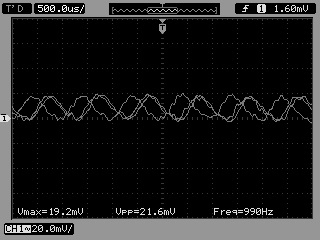
\includegraphics[scale=1]{imagens/acm.jpg} 
\centering
\caption{Tensão na saída para a medição do $A_{CM}$.}
\label{fig:acm} 
\end{figure} 

\begin{figure}[H] 
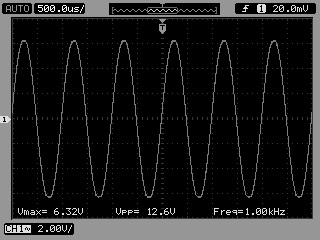
\includegraphics[scale=1]{imagens/ad.jpg} 
\centering
\caption{Tensão na saída para a medição do $A_{d}$.}
\label{fig:ad} 
\end{figure} 


Vide em anexo abaixo as folhas de cálculo utilizadas durante o experimento:

\begin{figure}[h!] 
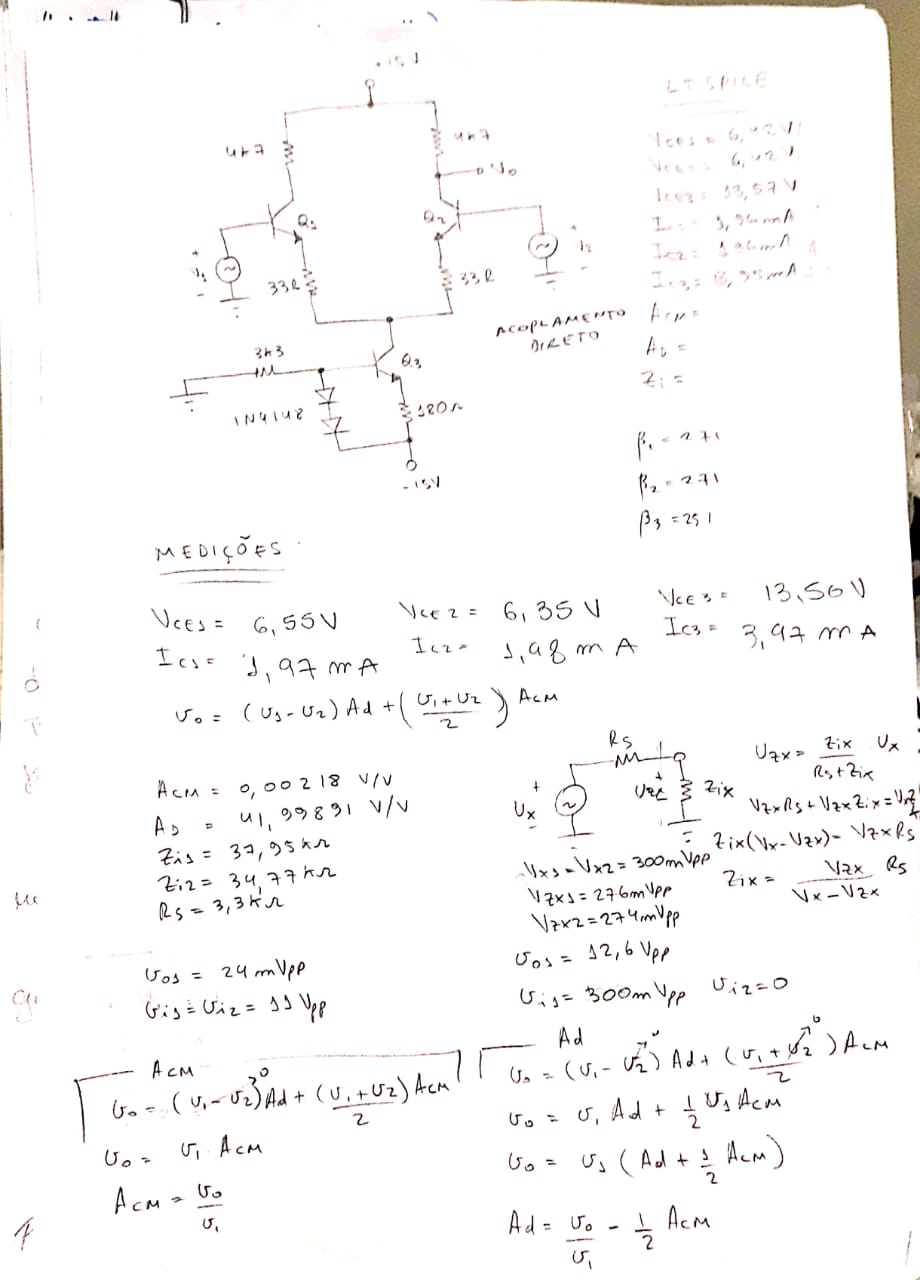
\includegraphics[scale=0.5]{imagens/scaner.jpeg} 
\centering
\caption{folha de cálculos.}
\label{calc:1} 
\end{figure} 





     






